Приведем в пример графки a(x), b(x), $P_{1}(i)$, с значенями, соотвествующими условиям (37).\\
Возьем следующие значения 	$N=2$ $r_{0}=0.7, r_{1}=0.2, r_{2}=0.1$, $\lambda$=0.8, $\mu_{1}$=0.6, $\mu_{2}$=1.5, q=0.25.

\begin{figure}[H]
	\centering
	\begin{minipage}[h]{0.49\linewidth}
		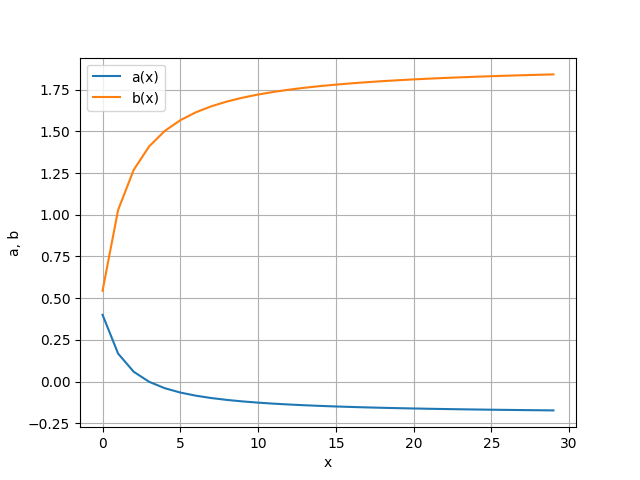
\includegraphics[width=0.8\linewidth]{ab2} 	
		\caption{Коэффициенты переноса и диффузии}
		\label{ris:experimoriginal}
	\end{minipage}
	\hfill
	\begin{minipage}[h]{0.49\linewidth}
		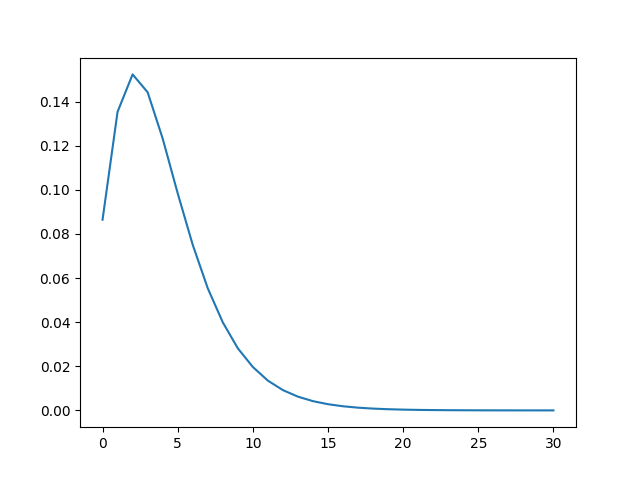
\includegraphics[width=0.8\linewidth]{P2} 
		\caption{Плотность распределения вероятностей числа заявок на орбите}
		\label{ris:experimcoded}
	\end{minipage}
\end{figure}

$N=10$ $r_{0}=0.7, r_{1}=0.2, r_{2}=0.1$, $\lambda$=0.8, $\mu_{1}$=0.6, $\mu_{2}$=1.5, q=0.25.
\begin{figure}[H]
	\centering
	\begin{minipage}[h]{0.49\linewidth}
		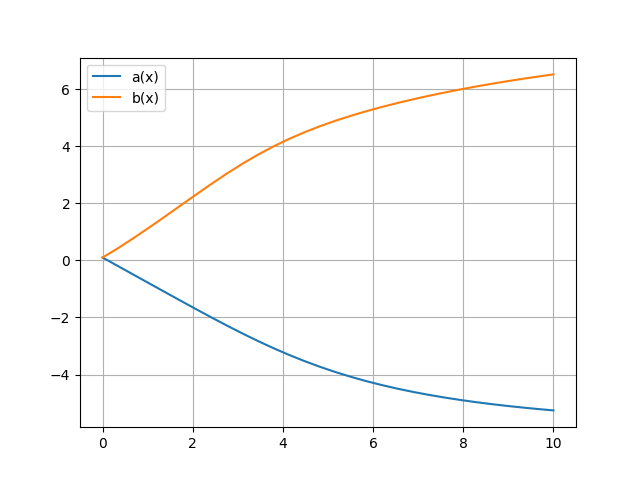
\includegraphics[width=0.8\linewidth]{ab10} 	
		\caption{Коэффициенты переноса и диффузии}
		\label{ris:experimoriginal}
	\end{minipage}
	\hfill
	\begin{minipage}[h]{0.49\linewidth}
		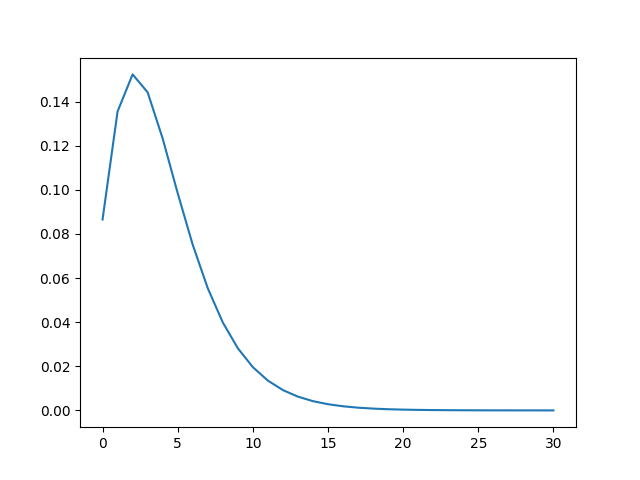
\includegraphics[width=0.8\linewidth]{P10} 
		\caption{Плотность распределения вероятностей числа заявок на орбите}
		\label{ris:experimcoded}
	\end{minipage}
\end{figure}

Данные графики были построены с помощью приложения Mathcad.
